\chapter{Einleitung}
\label{Einleitung}

\chapter{Benutzeroberfläche}
\label{Benutzeroberfläche}

\section{HTML zur Erstellung der Website}
\label{HTML zur Erstellung der Website}

\subsection{HTML-Formular Auswertung anhand einer Registrierung}
\label{HTML-Formular}

\section{CSS - Bootstrap}
\label{CSS - Bootstrap}

\subsection{Komaptibelität mit mobilen Endgeräten}
\label{Komaptibelität mit mobilen Endgeräten}

\section{Clientseitiges Javascript für benutzerspezifische Seiteninhalte}
\label{Clientseitiges Javascript}

\section{Anfahrtsbeschreibung per Google Maps}
\label{Anfahrtsbeschreibung per Google Maps}
Für den Fall, dass der Nutzer der Website von außerhalb des Ortes der Schule kommt, wurde eine Anfahrtbeschreibung mittels Google Maps eingebunden (siehe Abbildung \vref{fig:googleMaps}).

\begin{figure}[!htbp]
	\makebox[\textwidth]{ 
		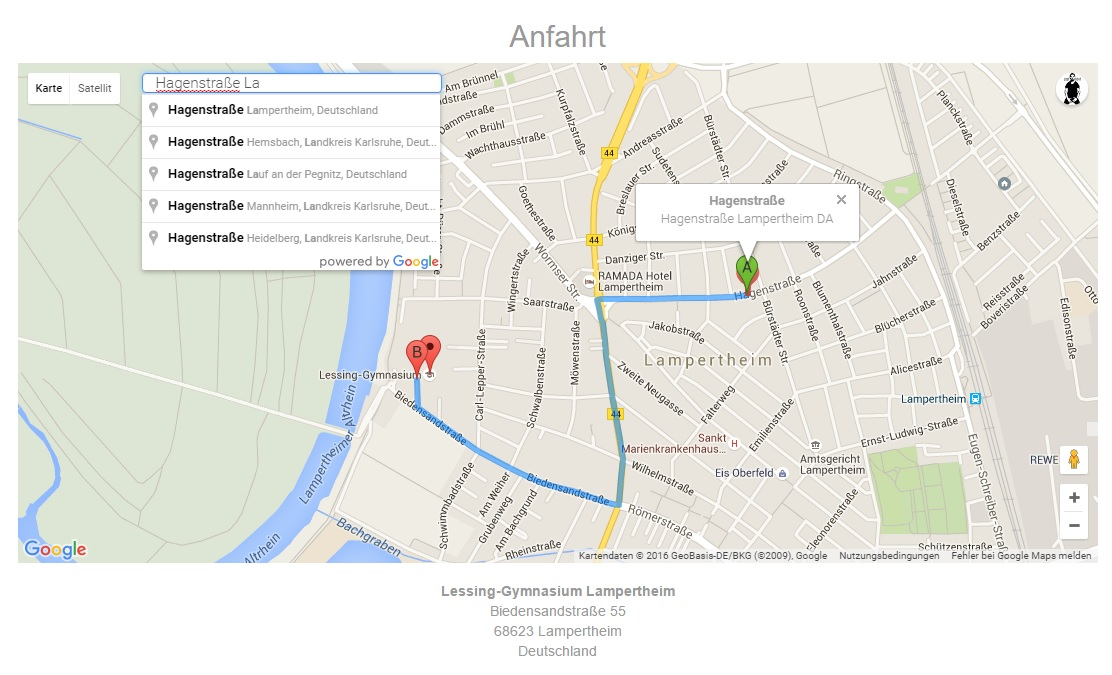
\includegraphics[scale=0.5]{img/googleMaps.jpg}}
	\caption{Anfahrtbeschreibung mit Google Maps}
	\label{fig:googleMaps}
\end{figure}

Auf dem Bild ist nicht nur der Standort der Schule vermerkt, sondern darüberhinaus kann der User über ein Eingabefeld links oben seine Abfahrtsadresse eingeben, sodass die optimale Route auf der Karte angezeigt wird. Des Weiteren wurde mit Hilfe der Autocomplete Funktion der Google Maps API eine automatische Vervollständigung der Adresse bei Eingabe in das Adressfeld implementiert, wie auf dem Screenshot zu sehen ist.
\par
Verwirklicht wurde die Einbindung, indem zuerst die Google Maps API und die Google Maps API für die Google Places per \textit{<script>}-Tag in den \textit{<head>} der Website importiert wurde (siehe Abbildung \vref{fig:googleMapsAPI}).

\begin{figure}[!htbp]
	\makebox[\textwidth]{ 
		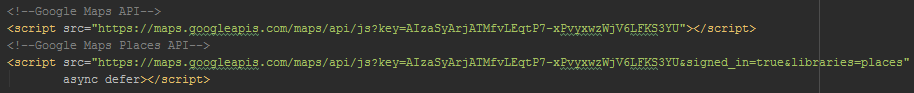
\includegraphics[scale=0.8]{img/googleMapsAPI.png}}
	\caption{API Einbindung von Google Maps}
	\label{fig:googleMapsAPI}
\end{figure}

Danach wird über eine JavaScript-Funktion, ebenfalls im <head>-Bereich die Map erstellt (siehe Abbildung \vref{fig:googleMapsInit}).

\begin{figure}[!bh]
	\makebox[\textwidth]{ 
		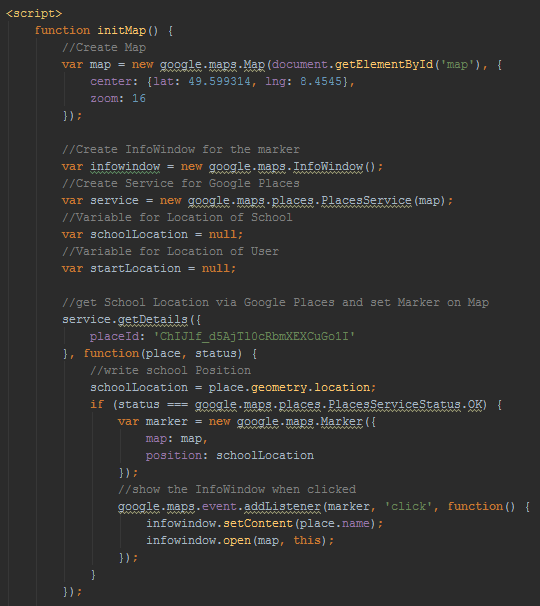
\includegraphics[scale=1]{img/googleMapsInit.png}}
	\caption{\textit{initMap}-Funktion zur Erstellung der Karte}
	\label{fig:googleMapsInit}
\end{figure}

Im zweiten Teil der selben Funktion wird die Autocomplete-Funktion für das Input-Feld implementiert und der Marker für die eingegebene Adresse auf der Karte gesetzt (siehe Abbildung \vref{fig:googleMapsInit2}).

\begin{figure}[!bh]
	\makebox[\textwidth]{ 
		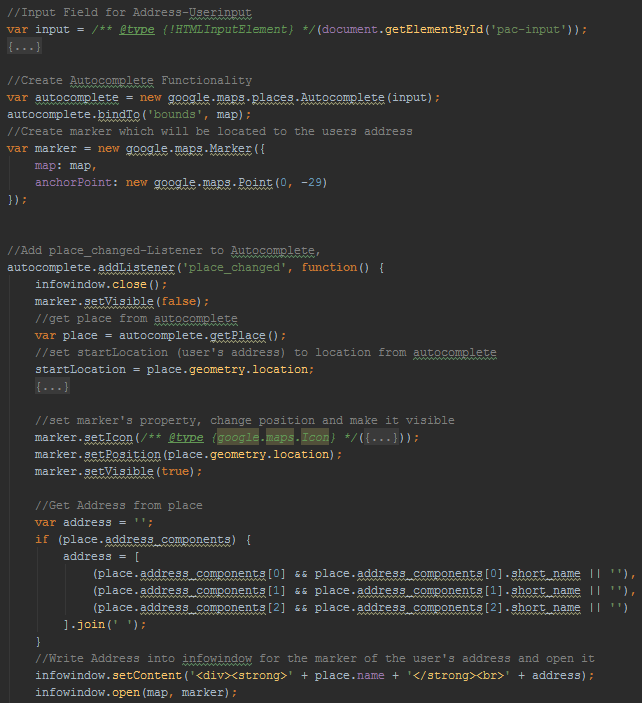
\includegraphics[scale=1]{img/googleMapsInit2.png}}
	\caption{Autocomplete-Funktion und Adressmarker}
	\label{fig:googleMapsInit2}
\end{figure}

Die Route zwischen der Abfahrtsadresse und der Schule wird im letzten Teil der Funktion erstellt und angezeigt. Vor Schließen des \textit{<script>}-Tags wird noch ein Event-Listener hinzugefügt, welcher auf das Aufrufen der Seite wartet und bei diesem dann die Karte zeichnet, indem dann die Funktion \textit{initMap} ausgeführt wird (siehe Abbildung \vref{fig:googleMapsInit3}).

\begin{figure}[!bh]
	\makebox[\textwidth]{ 
		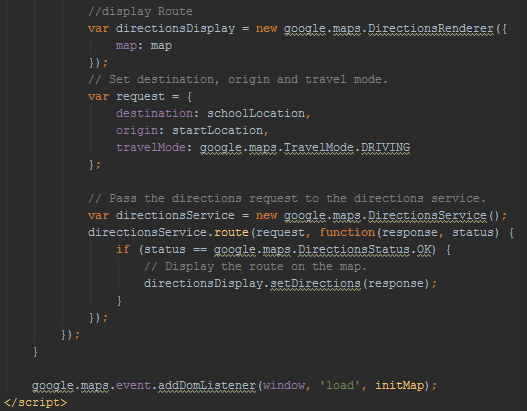
\includegraphics[scale=1]{img/googleMapsInit3.png}}
	\caption{Routenerstellung}
	\label{fig:googleMapsInit3}
\end{figure}

Um nun die Karte auch tatsächlich in der Website anzeigen zu können, wird zu guter Letzt noch \textit{div}-Container mit der Id \textit{"'map"'} an der Stelle, wo die Karte hingezeichnet werden soll, erstellt (siehe Abbildung \vref{fig:googleMapsDiv}). Dieses \textit{div} wird dann durch die Funktion \textit{initMap} gefüllt. Dafür wird bei Deklaration der Karte über einen Id-Selektor das entsprechende \textit{div} ausgewählt, in welchem die Google Map erscheinen soll (siehe Abbildung \vref{fig:googleMapsInit} (ganz oben)).

\begin{figure}[!bh]
	\makebox[\textwidth]{ 
		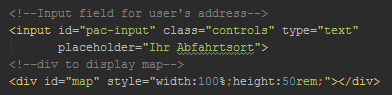
\includegraphics[scale=1]{img/googleMapsDiv.png}}
	\caption{Container für die Karte}
	\label{fig:googleMapsDiv}
\end{figure}

\section{Einbindung von Social Buttons mittels des Heise Plugins}
\label{Einbindung von Social Buttons mittels des Heise Plugins}
Um soziale Netzwerke der Schule oder des Sportfestes auf der Seite verlinken zu können, wurden mittels des Heise Plugins Social Buttons eingebunden (Facebook, Twitter und Google+). Der Vorteil bei diesem Plugin liegt darin, dass der Nutzer selbst bestimmen kann, ob er diese Buttons benutzen möchte, oder komplett für die Seite deaktivieren will. Der Sinn dahinter liegt in der Datenschutzproblematik bei der Einbindung der "`Like"'-Buttons von Facebook und Co.: Das Einbinden dieser Buttons erfolgt über einen iFrame, welcher von Facebook und Co. selbst zur Verfügung gestellt wird. Der iFrame enthält Code, der veranlasst, dass die URL der Seite, Cookies der Seite an Facebook geschickt wird. Ist der Anwender zudem gleichzeitig in einem anderen Fenster bei Facebook angemeldet, so schickt das iFrame zusätzlich Sitzungs-Id mit, wodurch Facebook einen Webseitenaufruf einer konkreten Person zuordnen kann.
\par
Damit das also nicht passiert, dürfte die Seite entweder keinerlei Elemente von Facebook, Twitter und Google+ behinhalten, oder das Heise Plugin verhindert eben genau dies, indem all diese Elemente zunächst bei Aufruf der Seite deaktiviert sind. Möchte der Nutzer nun einer der Funktionen der sozialen Netzwerke nutzen, so muss er die entsprechende erst über das Plugin aktivieren.
\par
In die Website integriert wurde das Plugin, indem zuerst das, von Heise zur Verfügung gestellte Skript des Plugins im \textit{<head>} geladen wird und ein HTML-Element durch ein weiteres Skript gefüllt wird (siehe Abbildung \vref{fig:heisePlugin1}).

\begin{figure}[!th]
	\makebox[\textwidth]{ 
		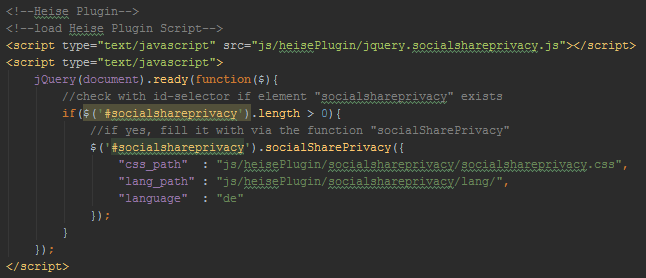
\includegraphics[scale=1]{img/heisePlugin1.png}}
	\caption{Integrieren des Heise Plugins}
	\label{fig:heisePlugin1}
\end{figure}

Durch ein \textit{div}-Element mit Id \textit{"'socialshareprivacy"'} (wie es in Abbildung \vref{fig:heisePlugin1} selektiert wird) vor dem Footer der Seite wird das Plugin dann am Ende der Seite angezeigt (siehe Abbildung \vref{fig:heisePlugin2}).

\begin{figure}[!bh]
	\makebox[\textwidth]{ 
		
\includegraphics[scale=1]{img/heisePlugin2.png}}
	\caption{Heise Plugin in der Website}
	\label{fig:heisePlugin2}
\end{figure}

\chapter{Client-Server-Kommunikation}
\label{Client-Server-Kommunikation}

\section{Anmeldefunktion per AJAX-Calls}
\label{Anmeldefunktion per AJAX-Calls}

\subsection{Bereitstellung eines REST-Service mit node.js}
\label{Bereitstellung eines REST-Service mit node.js}

\subsection{Konsumieren der Daten im Frontent mit AJAX-Calls}
\label{Konsumieren der Daten im Frontent mit AJAX-Calls}